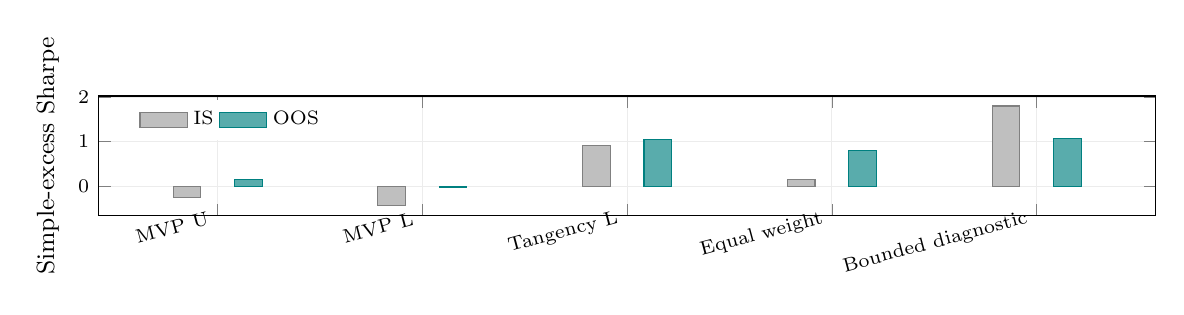
\begin{tikzpicture}\begin{axis}[width=15cm,height=5.1cm,tick label style={font=\scriptsize},label style={font=\small},legend style={font=\scriptsize,draw=none},scaled ticks=false,grid=major,grid style={gray!15},height=3.1cm,ylabel={Simple-excess Sharpe},xtick={0,1,2,3,4},xticklabels={MVP U,MVP L,Tangency L,Equal weight,Bounded diagnostic},x tick label style={font=\scriptsize,rotate=15,anchor=east},legend columns=2,legend pos=north west]
\addplot[ybar,area legend,bar shift=0pt,bar width=10pt,fill=gray!50,draw=gray] coordinates {(-0.150000,-0.263037) (0.850000,-0.436648) (1.850000,0.917358) (2.850000,0.153150) (3.850000,1.796878)};
\addlegendentry{IS}
\addplot[ybar,area legend,bar shift=0pt,bar width=10pt,fill=teal!65,draw=teal] coordinates {(0.150000,0.153683) (1.150000,-0.027496) (2.150000,1.052369) (3.150000,0.796231) (4.150000,1.059975)};
\addlegendentry{OOS}
\end{axis}\end{tikzpicture}
